


Geomecânica é o estudo das deformações e tensões em solos e rocha. Esse estudo se torna de extrema importância, pois, várias problemas podem ser solucionados através desses estudos, como:
\begin{itemize}
    \item Cálculo da pressão de fratura.
    \item Estabilidade de poços
\end{itemize}

Assim, simulações de geomecânicas são importantes para uma exploração segura do campo.

\section{Tensor de Tensões}

Para representar a tensão em um ponto da rocha, é utilizado um tensor de tensões de segunda ordem como segue abaixo:

\begin{equation}
\mathbf{\sigma} =
    \begin{bmatrix}
    \stxx & \stxy & \stxz \\
    \styx & \styy & \styz \\
    \stzx & \stzy & \stzz
    \end{bmatrix}
\end{equation}

O primeiro subscrito do tensor representa a face que a tensão está sendo aplicada, enquanto o segundo representa a direção da tensão. A figura \ref{fig:tensoesx} mostra as componentes com o com primeiro subscrito x.


\begin{figure}[!htbp]
\centering
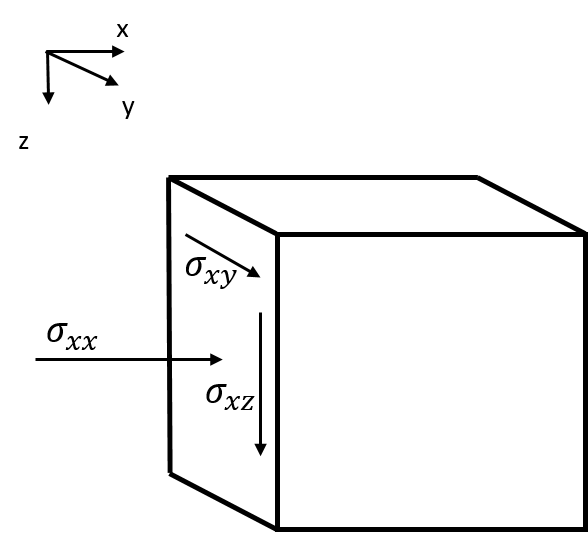
\includegraphics[width=5cm]{chap01/tensor.png}
\caption{Tensões $\sigma_{x.}$ representadas graficamente.}
\label{fig:tensoesx}
\end{figure}

Ao aplicar a condição de equilíbrio do momento, chega-se a conclusão que $\stxy=\styx$, $\stxz=\stzx$ e $\styz=\stzy$. Dessa maneira, para a representação desse tensor, são necessários guardar apenas seis valores. Dessa forma, pode-se considerar a tensão como o vetor apresentado \label{eq:tensor6} essa notação é chamada de notação de Voigt e é a bastante utilizada nas implementações de elementos finitos, por exemplo, nas formulações apresentadas por \cite{hughes} e \cite{jacob}.


\begin{equation}
\sigma^T = \begin{bmatrix}
\stxx & \styy & \stzz & \stxy & \stxz & \styz
\end{bmatrix}
\label{eq:tensor6}
\end{equation}


\section{Teoria da Consolidação}

Para um certo elemento de volume $\Delta x\Delta y \Delta z$, representado na figura \ref{fig:equilibrio}, pode-se escrever o equilíbrio nas direções x, y e z.

\begin{figure}[!htbp]
\centering
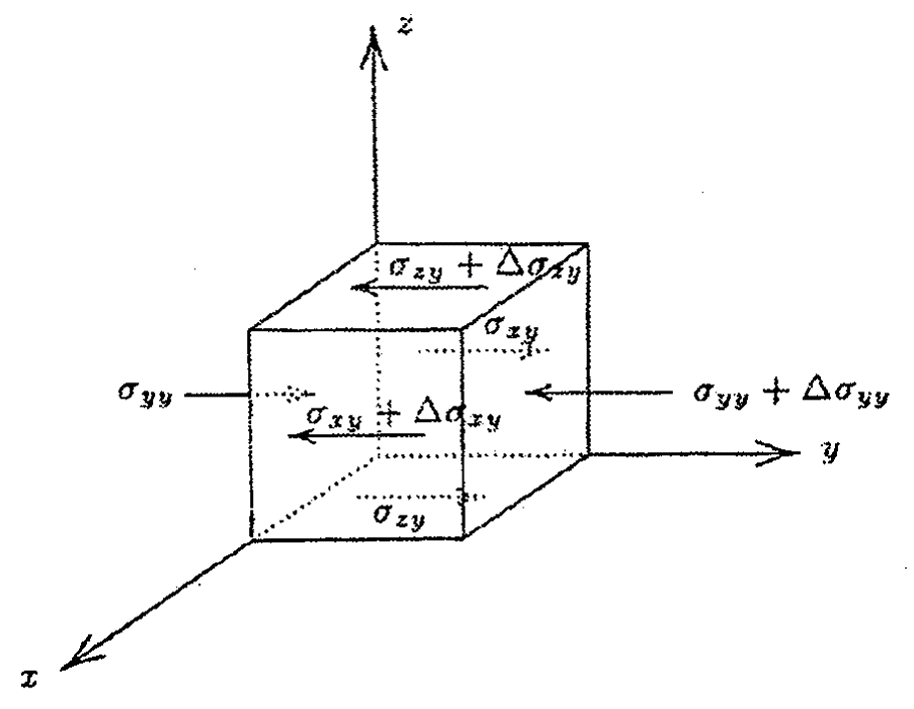
\includegraphics[width=6cm]{chap01/equilibrio.png}
\caption{Tensões na direção y ($\sigma_{.y}$) representadas graficamente.  Fonte: \cite{CompGeomec}}
\label{fig:equilibrio}
\end{figure}

Para a direção y, por exemplo, tem-se:

\begin{multline}
   (\stxy - \stxy - \Delta \stxy) \Dy\Dz + (\styy - \styy - \Delta \styy)\Dx\Dz  +\\
   + (\stzy - \stzy - \Delta\stzy) \Dx\Dy + f_y\Dx\Dy\Dz = 0
\end{multline}

\begin{equation}
 \Delta \stxy \Dy\Dz + \Delta \styy\Dx\Dz + \Delta\stzy - f_y\Dx\Dy\Dz = 0
\end{equation}

\begin{equation}
\dx[\stxy] + \dy[\styy] + \dy[\stzy] - f_y = 0
\end{equation}

Analogamente, para as outras direções, pode-se montar o seguinte sistema de equações de equilíbrio.

\begin{equation}
\label{eq:equilibrio1}
\left\{\begin{matrix}
 \dx[\stxx] + \dy[\styx] + \dz[\stzx] - f_x & = & 0\\
 \dx[\stxy] + \dy[\styy] + \dz[\stzy] - f_y & = & 0\\
 \dx[\stxz] + \dy[\styz] + \dz[\stzz] - f_z & = & 0
\end{matrix}\right.
\end{equation}

As tensões apresentadas nas equações \ref{eq:equilibrio1} são as atuam no bloco infinitesimal. Acontece que ao tratar de reservatórios de petróleo, estes possuem fluído no volume poroso da rocha (óleo ou água) e, portanto, parte da tensão será suporta pelo fluído e parte será suportado pelos grãos da rocha. Como fluído não oferece resistência ao cisalhamento, ele suporta apenas parte das tensões $\stxx$, $\styy$ e $\stzz$.

Experimentalmente foi constado por Biot em que a equação que rege a tensão efetiva na rocha ($\sigma^{\prime\prime}$) é dada pela equação \ref{eq:tensaoefetiva} (veja \cite{ResGeomec} cap 02).

\begin{equation}
\label{eq:tensaoefetiva}
    \sigma^{\prime\prime} = \sigma - \alpha P_p
\end{equation}

Onde $\alpha$ é o coeficiente de biot e $P_p$ a pressão de poros. O coeficiente de biot representa o quanto a pressão de poros do fluído suporta a tensão total na rocha, portanto, $\alpha \in [0,1]$.

Assim, as equações \ref{eq:equilibrio1} podem ser reescritas como \ref{eq:equilibrio} substituindo a tensão total $\sigma$ pela tensão efetiva na rocha ($\sigma^\prime$). Essas equações são encontras em \cite{CompGeomec}.



\begin{equation}
\label{eq:equilibrio}
\left\{\begin{matrix}
\dx[\sxx]  + \dy[\syx] + \dz[\szx] + \dx[\alpha P_p] - f_x   = 0
\\
\dx[\sxy]  + \dy[\syy] + \dz[\szy] + \dy[\alpha P_p]  - f_y   = 0
\\
\dx[\sxz]  + \dy[\syz] + \dz[\szz] + \dz[\alpha P_p] - f_z   = 0
\end{matrix}\right.
\end{equation}

Ou ainda, escrevendo de forma matricial.

\begin{equation}
\label{eq:equilibrio_matriz}
\nabla \cdot \sigma^\prime - \nabla \alpha P_p - f = 0
\end{equation}

Onde $f^T=\begin{bmatrix}f_x & f_y & f_z\end{bmatrix}$.


Por motivos de implementação mais eficiente menor uso de memória e utilização de operações mais simples (multiplicação de matrizes por vetores) a equação acima pode ser escrita na notação de Voigt que considerando as definições abaixo:

\begin{equation}
\begin{matrix}
\sigma^\prime = \begin{bmatrix}
\sxx
\\
\syy
\\
\szz
\\
\sxy
\\
\sxz
\\
\syz
\end{bmatrix}
&

;

&

f = \begin{bmatrix}
f_{x}
\\
f_{y}
\\
f_{z}
\end{bmatrix}
&
;
&

m = \begin{bmatrix} 1 \\ 1 \\ 1 \\ 0 \\ 0 \\ 0\end{bmatrix}

&
;

&
\sopnabla = \sop
\end{matrix}
\end{equation}

A equação \ref{eq:equilibrio_matriz} pode ser reescrita como \ref{eq:equilibrio_final}.

\begin{equation}
\label{eq:equilibrio_final}
\sopnabla^T\sigma^{\prime\prime} - \sopnabla^T\alpha m  P_p - f = 0
\end{equation}


\subsection{Relações Constitutivas}

\textit{"Uma relação constitutiva descreve a deformação de uma rocha em resposta a uma tensão (e vice-versa)."} \cite{ResGeomec}


Vários tipos de leis constitutivas podem ser utilizadas para representar essa relação entre tensão e deformação. A figura \ref{fig:stress_strain} mostram dados de um teste típico de tensão-deformação em uma rocha bem cimentada. Nesse caso, é importante notar que o comportamento linear é a região dominante nesse tipo de teste. Essa região onde as deformações e tensões se relacionam linearmente é chamada de elástica.


\begin{figure}[!htbp]
\centering
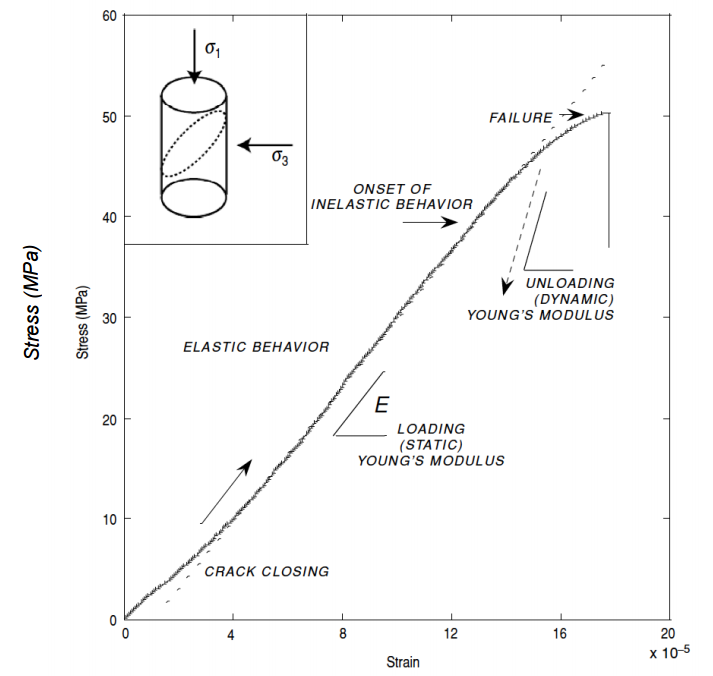
\includegraphics[width=7cm]{chap01/stress_strain.PNG}
\caption{Teste de laboratório tensão-deformação para uma rocha bem cimentada. Fonte: \cite{ResGeomec}}
\label{fig:stress_strain}
\end{figure}


O estudo de mecânica dos sólidos nos mostra que, na região elástica e materiais isotrópicos, é possível escrever uma relação entre as deformações e tensões nos elementos de forma simples. Essa relação é denominada de Lei de Hooke Generalizada e é apresentada na Equação \eqref{eq:hooke}. E a Equação \eqref{eq:elasticMatrix} apresenta a matriz de elasticidade.


\begin{equation}{
\label{eq:hooke}
\fontsize{4}{4}\selectfont
\sigma ^{\prime\prime}= D \epsilon
}
\end{equation}



Onde $E$ é o módulo de Young da rocha e $v$ o módulo de de Poisson. Já as deformações se relacionam com os deslocamentos pela equação \eqref{eq:defor_desloc}.

\begin{equation}
\label{eq:defor_desloc}
\epsilon = \sopnabla u
\end{equation}


A EDP da equação \eqref{eq:equilibrio_final} pode então ser escrita em função dos deslocamentos substituindo as equações \eqref{eq:hooke} e \eqref{eq:defor_desloc}.

\begin{equation}
\label{eq:edp_geomec}
\sopnabla^TD \sopnabla u - \sopnabla^T\alpha m P_p - f = 0
\end{equation}

Onde $D$ é a matriz de elasticidade da Lei de Hooke. Essa forma será a utilizada junto dos métodos do elementos finitos para construção de um simulador para regime permanente de geomecânica em duas dimensões. Ao se passar
de três dimensões para duas dimensões existem duas abordagens possíveis de stress plano ou deformação plana. Que são apresentadas respectivamente em \eqref{eq:elasticplanestress} e \eqref{eq:elasticplanestrain}.

\begin{equation} \label{eq:elasticplanestress}
D_{stress} = \frac{E}{1-\upsilon^2}
\begin{bmatrix}
1  & \upsilon & 0 \\ 
\upsilon & 1 &  0 \\ 
0 & 0 & \frac{1-\upsilon}{2}
\end{bmatrix}
\end{equation}

\begin{equation} \label{eq:elasticplanestrain}
D_{strain} = \frac{E}{(1+\upsilon)(1-2\upsilon)}
\begin{bmatrix}
 1-\upsilon & \upsilon    &  0 \\ 
 \upsilon   &  1-\upsilon &  0 \\ 
 0& 0 & \frac{1-2\upsilon}{2}
\end{bmatrix}
\end{equation}

De acordo com \cite{jacob}, a condição de deformação plana é melhor aplicada quando o elemento é grosso em relação ao plano xy que é o caso dos reservatórios de petróleo.  Dessa forma, artigos como \cite{planeStrainProblems}, \cite{casteletto} e \cite{irina} utilizam a hipótese de deformação plana que será a mesma utilizada nesse trabalho.

Os operadores e vetores devem então ser redefinidos para os mostrados em \eqref{eq:vetores2d}.

\begin{equation}
\label{eq:vetores2d}
\begin{matrix}
\sigma^\prime = \begin{bmatrix}
\sxx
\\
\syy
\\
\sxy
\end{bmatrix}
&

;

&

f = \begin{bmatrix}
f_{x}
\\
f_{y}
\end{bmatrix}
&
;
&

m = \begin{bmatrix} 1 \\ 1 \\ 0\end{bmatrix}

&
;

&
\sopnabla = \soptwod

&
;

&

u = \begin{bmatrix}
u_x
\\ 
u_y
\end{bmatrix}

\end{matrix}
\end{equation}

Além da Equação \eqref{eq:edp_geomec}, são necessárias as condições de contorno para que o problema fique totalmente definido. 
